
\section{Multiclass Kernel SVMs}


\subsection{Multiclass SVM strategies}

\subsubsection{spoc-svc}

This method for multi-class classification is based on a new definition of the margin. This generalized notion of margin gives to the method the ability to learn a multi-class classifier simply by solving a constrained optimization
problem with a quadratic objective function.

See \cite{spoc-svc} for more details.


\subsubsection{kbb-svc}

In this case, we extend the binary SVM optimisation problem by adding new decision variables and new constraints. This method implies that the size of the optimisation problem is proportional to the number categories, which can be a problem. 

See \cite{kbb-svc} for more details.


\subsubsection{one-vs-all approach}


\subsubsection{tree-based approach}



\subsection{Parameter optimization}

\subsubsection{spoc-svc}

\subsubsection{kbb-svc}

\subsubsection{one-vs-all approach}

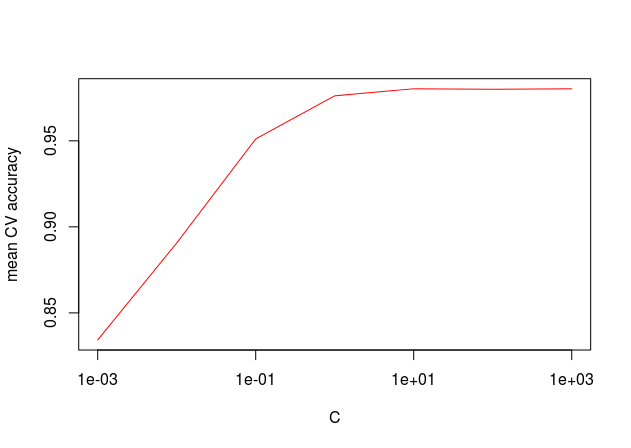
\includegraphics[width=0.8\textwidth]{../plots/one_vs_all_zip}

\subsubsection{tree-based approach}


\subsection{Results}